\documentclass{article}
\usepackage[utf8]{inputenc}
\usepackage{amsthm}
\usepackage{amsmath}
\usepackage{amssymb}
\usepackage{tikz}
\usepackage{authblk}
\usepackage{mathtools}

\usetikzlibrary{calc,shapes.geometric, decorations.pathreplacing}

\newtheorem*{definition}{Definition}
\newtheorem*{proposition}{Proposition}
\newtheorem*{lemma}{Lemma}
\newtheorem*{corollary}{Corollary}

\newcommand{\R}{\mathbb{R}}
\newcommand{\pwrset}{\mathcal{P}}

\newcommand{\B}{\mathcal{B}}
\newcommand{\bcup}{\cup}
\newcommand{\bcap}{\Cap}
\newcommand{\bstar}{^\circledast}
\newcommand{\bcont}{\mathcal{C}^\R}
\newcommand{\bmeasure}{\leq_\mu^\R}

\newcommand{\lang}{\mathcal{L}}
\newcommand{\Vars}{\text{Vars}}
\newcommand{\Pol}{\text{Pol}}


\newcommand{\lcup}{\sqcup}
\newcommand{\lcap}{\sqcap}
\newcommand{\lstar}{^*}
\newcommand{\lpart}{\sqsubseteq}
\newcommand{\lcont}{C}
\newcommand{\lmeasure}{\preceq}

\newcommand{\eqdef}{\stackrel{\text{def}}{=}}
\newcommand{\eqih}{\stackrel{\text{ i.h.}}{=}}
\newcommand{\equivih}{\stackrel{\text{i.h.}}{\leftrightarrow}}

\title{Axiomatization of Some Contact Logics with a Qualitative Measure}
\author{Anguel Nikolov\\{\small supervised by Prof. Tinko Tinchev}}
\affil{Faculty of Mathematics and Informatics \\
  Sofia University ``St. Kliment Ohridski''}
\date{\today}

\begin{document}

\maketitle

\section{Introduction}

The aim of this work is to explore the axiomatization and decidability of the quantifier-free theories of a structure, which arises from a certain kind of geometric objects on the real line. Three relations between these objects are considered: parthood, contact and qualitative measure.

The objects are referred to as polytopes, though they are in fact unions of what may usually be understood by the term. A key property by which they are chosen is that they have a true interior.

The parthood relationship between these objects gives rise to a Boolean algebra and two further relations are considered: contact and qualitative measure.
\section{Notation and Notions}
Listed below are some well-established notions and the notation for them in this text.
\begin{itemize}
\item $\R$ denotes the real numbers, $\R^+$ the positive real numbers and $\R^+_0$ the non-negative ones.
\item $-\infty$ and $\infty$ are the least and greatest elements of $\R \cup \{-\infty, \infty\}$.
\item For the purposes of measure, the $+$ operation over $\R^+_0$ is extended in the usual way:
  \begin{equation*}
    r + \infty \eqdef \infty + r \eqdef \infty \text{, for any } r \in \R^+_0 \cup \{\infty\}
  \end{equation*}
\item $\pwrset(X)$ denotes the set of all subsets of $X$.
\item TODO: Closure and interior
\item TODO: Graph, Cycle
\item TODO: Tree, Rooted Tree, Children(T, u), SubTree(T, v)
\end{itemize}
\section{Language}
This section describes the language, whose semantics we will consider in a couple of contexts.

\begin{definition}[Language]
$\lang$ denotes the first-order language of only quantifier-free formulas, which contains the following non-logical symbols:
\begin{itemize}
  \item predicate symbols:
  \begin{itemize}
  \item binary infix $\lpart$: parthood
  \item binary infix $\lmeasure$: measure comparison
  \item binary prefix $\lcont$: contact
  \end{itemize}
  \item functional symbols:
  \begin{itemize}
  \item binary infix function $\lcup$: union
  \item binary infix function $\lcap$: intersection
  \item unary postfix function $\lstar$: complement
  \end{itemize}
  \item constant symbols:
  \begin{itemize}
  \item $0$: empty polytope
  \item $1$: universe
  \end{itemize}
\end{itemize}

The logical symbols $\land$, $\lor$, $\lnot$, $\Rightarrow$, $\top$, $\bot$ are used in the usual way and the set of individual variables is denoted $\Vars$.

\end{definition}

\section{Semantics}

Though the aim is to interpret the language on the real line, other models will also be needed. It is beneficial fix their common semantics, which are defined below in the expected way.

Let $\B$ be a Boolean algebra with carrier $B$ and $\mathcal{C}$ and $\mathcal{M}$ be relations over $B$. Further, $S = \langle \B, \mathcal{C}, \mathcal{M} \rangle$.

\begin{definition}[Value of a Term in $S = \langle \B, \mathcal{C}, \mathcal{M} \rangle$]
  Let $v: \Vars \rightarrow B$. Then,  $v^S$ denotes the extension of $v$ to the terms of $\lang$ in the following structurally recursive way:
  \begin{itemize}
  \item $v^S(0)$ is the zero of $\B$
  \item $v^S(1)$ is the unit of $\B$
  \item $v^S(\tau_1 \lstar)$ is the complement of $v(\tau_1)$ in $\B$,
  \item $v^S(\tau_1 \lcup \tau_2)$ is the join of $v(\tau_1)$ and $v(\tau_2)$ in $\B$,
  \item $v^S(\tau_1 \lcap \tau_2)$ is the meet of $v(\tau_1)$ and $v(\tau_2)$ in $\B$,
  \end{itemize}
for any terms $\tau_1$ and $\tau_2$ of $\lang$.

\end{definition}

\begin{definition}[Validity of a Formula in $S = \langle \B, \mathcal{C}, \mathcal{M} \rangle$]
  Again, let $v: \Vars \rightarrow B$. Validity of a formula $\phi$ in $S$ with valuation $v$ is denoted $\langle S, v \rangle \models \phi$ and defined over elementary formulas like so:
  \begin{itemize}
  \item $\langle S, v \rangle \models \tau_1 \lpart \tau_2 \longleftrightarrow v^S(\tau_1)$ is less than or equal to $v^S(\tau_2)$ in $\B$,
  \item $\langle S, v \rangle \models \lcont(\tau_1, \tau_2) \longleftrightarrow \mathcal{C}(v^S(\tau_1), v^S(\tau_2))$,
  \item $\langle S, v \rangle \models \tau_1 \lmeasure \tau_2 \longleftrightarrow \mathcal{M}(v^S(\tau_1), v^S(\tau_2))$,
  \end{itemize}
  for any terms $\tau_1$ and $\tau_2$ of $\lang$. For complex formulas, the extension is done in the usual way:
  \begin{itemize}
  \item $\langle S, v \rangle \models \top$ and $\langle S, v \rangle \not \models \bot$,
  \item $\langle S, v \rangle \models \lnot \phi \longleftrightarrow \langle S, v \rangle \not\models \phi$,
  \item $\langle S, v \rangle \models \phi \land \psi \longleftrightarrow \langle S, v \rangle \models \phi$ and $\langle S, v \rangle \models \psi$,
  \item $\langle S, v \rangle \models \phi \lor \psi \longleftrightarrow$ at least one of  $\langle S, v \rangle \models \phi$ and $\langle S, v \rangle \models \psi$ holds,
  \end{itemize}
  where $\phi$ and $\psi$ are (quantifier-free) formulas of $\lang$.

  If $\langle S, v \rangle \models \phi$ for all $v: \Vars \rightarrow B$, then $S \models \phi$.
\end{definition}

\subsection{Polytopes on the Real Line}

A specific kind of objects will be considered: finite unions of closed, potentially infinite, intervals on the real line. These are defined below, along with the operations and properties with which the language will be concerned.

\begin{definition}[Basis Polytope]
For any $m$, $n \in \R$ such that $m < n$, the intervals $[m, n]$, $(-\infty, m]$, $[m, \infty)$ and $(-\infty, \infty)$ are called \emph{basis polytopes}.
\end{definition}

\begin{definition}[Polytope]
For any finite set of basis polytopes $B$, $\bigcup B$ is called a \emph{polytope}. The set of all polytopes is denoted $\Pol(\R)$.
\end{definition}

Remark that for $B = \emptyset$, the empty set is also a polytope.

\begin{proposition}
Any non-empty polytope can be uniquely represented as the union of a finite set of non-intersecting basic polytopes.
\end{proposition}
\begin{proof}
  TODO: write proof
\end{proof}

\begin{definition}(Standard Representation)
The set from the above proposition is called the \emph{standard representation} of a polytope.
\end{definition}

\begin{definition}[Polytope Operations]
For any polytopes $p$ and $q$, we define the following operations as modifications of intersection and complement:
\begin{itemize}
  \item $p \bcap q \eqdef Cl(Int((p \cup q)))$;
  \item $p \bstar \eqdef Cl(\R \setminus p) $.
\end{itemize}
The union operation $p \bcup q$ will be considered in the same context, though no modification is needed.
\end{definition}

The modification of union ensures that there are no isolated points and the modification of complement ensures that results of the operations remain a union of \emph{closed} intervals.

\begin{proposition}
$\Pol(\R)$ forms a Boolean algebra with
  \begin{itemize}
  \item $\subseteq$ for Boolean inequality,
  \item $\bcap$ for meet,
  \item $\bcup$ for join,
  \item $\bstar$ for complement,
  \item $\emptyset$ for the zero and
  \item $\R$ for the unit.
\end{itemize}
This algebra will be denoted $\B^\R$.
\end{proposition}
\begin{proof}
  TODO: write proof
\end{proof}

\begin{proposition}
  $\B^\R$ is incomplete.
\end{proposition}
\begin{proof}
  TODO: write proof
\end{proof}

\begin{definition}[Line Contact]
Two polytopes $p$ and $q$ are \emph{in contact} if $p \cap q \neq \emptyset$. This is denoted $\bcont(p, q)$.
\end{definition}

\begin{definition}[Polytope Measure]
  The measure of a basic polytope of the kind $[m, n]$, for $m, n \in \R$ is $n-m$. The measure of a basic polytope with an infinite bound is $\infty$.

  The \emph{measure} of a polytope $p$, denoted $\mu^\R(p)$, is the sum of the measures of the basic polytopes of its standard representation.

The \emph{qualitative measure relation induced by} $\mu^\R$ is defined
\begin{equation*}
  p \bmeasure q \longleftrightarrow \mu^\R(p) \leq \mu^\R(q),
\end{equation*}
  for any $p, q \in \Pol(\R)$.
\end{definition}

\begin{proposition}
  $\mu^\R$ is a measure.
\end{proposition}
\begin{proof}
  TODO: write proof
\end{proof}

$\mu^\R$ is a restriction of the usual measure on $\R$.

\begin{proposition}
The only polytope with measure $0$ is $\emptyset$. Further, every non-zero polytope has an arbitrary small non-zero sub-polytope. Consequently, $\B^\R$ is atomless.
\end{proposition}
\begin{proof}
  TODO: write proof
\end{proof}

Given the definition of $\B^\R$, measure and contact above, the model on the real line is defined directly:

\begin{definition}[Real Line Model]
  \begin{equation*}
    S^\R \eqdef \langle \B^\R, \bcont, \bmeasure \rangle
  \end{equation*}
\end{definition}

\subsection{Relational Models}
In order to find appropriate value functions for a well chosen kind of formulas, an abstraction model will be needed. It is quite generic, yet it turns out to be easily transformed into an equivalent real line model, given some constraints.

Let $W$ be a finite set and $\B^W$ be the Boolean algebra of all subsets of $W$. Let $c$ be an arbitrary symmetric and reflexive relation over $W$ and $m: W \rightarrow \R^+ \cup \{\infty\}$.

Let $\mathcal{C}^c$ be the relation over $\pwrset(W)$ defined as
\begin{equation*}
  \mathcal{C}^c(a, b) \longleftrightarrow (\exists i \in a)(\exists j \in b)(\langle i, j \rangle \in c)
\end{equation*}
Let $\mu^m: \pwrset(W) \rightarrow \R_0^+ \cup \{\infty\}$ such that:
\begin{equation*}
  \mu^m(a) \eqdef \sum_{i \in a}m(i)
\end{equation*}
And finally, let $\leq_m$ be the relation over $\pwrset(W)$:
\begin{equation*}
  a \leq_m b \longleftrightarrow \mu^m(a) \leq \mu^m(b),
\end{equation*}
all for $a$, $b \subseteq W$.
\begin{definition}[Relational Model]
$\langle \B^W, \mathcal{C}^c, \leq_m \rangle$ is called the \emph{relational model for $W$, $c$ and $m$}.
\end{definition}

\subsubsection{Converting to a Real Line Model}
Relational models are useful because they can be converted to real line models under certain conditions.
\begin{definition}[Contact Graph]
  Let $S = \langle \B^W, \mathcal{C}^c, \leq_m \rangle$ be a relational model. Let $E$ denote the set of pairs of different vertices in $c$, but unordered: $E \eqdef \{\, \{i, j\} \mid \langle i, j \rangle \in c$ \& $i \neq j \,\}$. Note that since $c$ is reflexive and symmetric, no information is lost when obtaining $E$ from $c$.
  The graph $\langle W, E \rangle$ is called the \emph{contact graph of $S$} and denoted $Gr(S)$.
\end{definition}
\begin{definition}[Convertible Relational Model]
Let $S = \langle \B^W, \mathcal{C}^c, \leq_m \rangle$ be a relational model and suppose that the following constraints hold:
\begin{itemize}
\item $Gr(S)$ is connected and
\item there are exactly two elements of $W$ with infinite values for $m$, i.e. there exist $i \in W$ and $j \in W$, $i \neq j$ such that:
  \begin{equation*}
    m(i) = m(j) = \infty \text{ and } (\forall k \in W \setminus \{i, j\})(m(k) \neq \infty).
  \end{equation*}
\end{itemize}
Then, $S$ is called a \emph{convertible relational model}.
\end{definition}

\begin{definition}[Disjoint Valuation]
  Suppose $S = \langle \B^W, \mathcal{C}^c, \leq_m \rangle$ is a convertible relational model and $v: \Vars \rightarrow \pwrset(W)$ such that
\begin{equation*}
(\forall x \in \Vars)(\forall y \in \Vars)(v(x) \neq v(y) \rightarrow v(x) \cap v(y) = \emptyset).
\end{equation*}
Then, $v$ is called a \emph{disjoint valuation}.
\end{definition}

Although a valuation is an infinite object, any given formula contains a finite number of variables. Therefore, only a finite part of the valuation is relevant to the truth value of that formula. The effective construction of a valuation as discussed below is possible because the valuation will always be considered in the context of a formula and will therefore be encodable by a finite object.

\begin{lemma}[Untying]
  Let $S = \langle \B^W, \mathcal{C}^c, \leq_m \rangle$ be a convertible relational model and $v$ be a disjoint valuation. Suppose $Gr(S)$ is not a tree.
  Then, there is a procedure to effectively construct a convertible relational model $S'$ and a disjoint valuation $v'$ for $S'$ such that:
  \begin{itemize}
  \item $Gr(S')$ has one vertex more and the same number of edges and
  \item for any formula $\phi$ in $\lang$, $\langle S, v \rangle \models \phi \longleftrightarrow \langle S', v' \rangle \models \phi$.
  \end{itemize}
\end{lemma}
\begin{proof}
  Given that $Gr(S)$ is not a tree, yet is connected, it must contain at least one cycle. A cycle can be effectively found using a depth-first search. Let $\pi$ be such a cycle.

  Let $i$ and $j$ be any two consecutive vertices in $\pi$ such that $m(i) \neq \infty$. This requirement is always achievable, since there are at least three vertices in a cycle and exactly two vertices with infinite values for $m$ in a convertible relational model. Therefore, there will be at least one vertex with a finite value for $m$ in any cycle.

  The aim is to disconnect $\pi$ by removing the edge between $i$ and $j$. In order to achieve that, intuitively, the portion of $i$ which is in contact only with $j$ will be separated out into a separate atomic object, $i'$, having half the measure.

\begin{figure}[ht]
    \centering
    \begin{minipage}{0.45\textwidth}
      \centering
      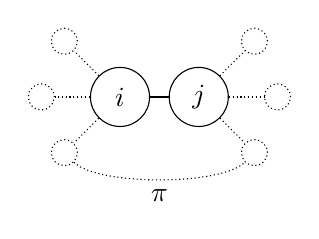
\begin{tikzpicture}[main/.style = {draw, circle, minimum size=.75cm},
          small/.style = {draw, densely dotted, circle, minimum size=.25cm},
          dedge/.style = {densely dotted}]
        \node[main] (i) {$i$};
        \node[main] (j) [right of=i] {$j$};
        \node[small] (i1) [below left of=i] {};
        \node[small] (i2) [above left of=i] {};
        \node[small] (i3) [left of=i] {};
        \node[small] (j1) [below right of=j] {};
        \node[small] (j2) [above right of=j] {};
        \node[small] (j3) [right of=j] {};
        \draw (i) -- (j);
        \foreach \n in {i1, i2, i3}
                 {
                   \draw[dedge] (i) -- (\n);
                 }
        \foreach \n in {j1, j2, j3}
                 {
                   \draw[dedge] (j) -- (\n);
                 }
        \draw[dedge] (i1) to [out=315, in=225, looseness=.5] node[midway, below] {$\pi$} (j1);
      \end{tikzpicture}
    \end{minipage}$\rightsquigarrow$
    \begin{minipage}{0.45\textwidth}
      \centering
      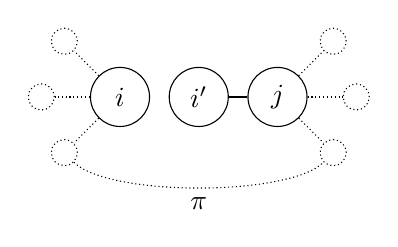
\begin{tikzpicture}[main/.style = {draw, circle, minimum size=.75cm},
          small/.style = {draw, densely dotted, circle, minimum size=.25cm},
          dedge/.style = {densely dotted}]
        \node[main] (i) {$i$};
        \node[main] (i') [right of=i] {$i'$};
        \node[main] (j) [right of=i'] {$j$};
        \node[small] (i1) [below left of=i] {};
        \node[small] (i2) [above left of=i] {};
        \node[small] (i3) [left of=i] {};
        \node[small] (j1) [below right of=j] {};
        \node[small] (j2) [above right of=j] {};
        \node[small] (j3) [right of=j] {};
        \draw (i') -- (j);
        \foreach \n in {i1, i2, i3}
                 {
                   \draw[dedge] (i) -- (\n);
                 }
        \foreach \n in {j1, j2, j3}
                 {
                   \draw[dedge] (j) -- (\n);
                 }
%        \draw[dedge] (i1)  (j1);
        \draw[dedge] (i1) to [out=315, in=225, looseness=.5] node[midway, below] {$\pi$} (j1);
      \end{tikzpicture}
    \end{minipage}
\end{figure}

  Let $i' \not \in W$ and let:
\begin{align*}
W' &\eqdef W \cup \{i'\} \\
c' &\eqdef (c \setminus \{\langle i, j \rangle, \langle j, i \rangle\}) \cup \{\langle i', j \rangle, \langle j, i' \rangle, \langle i', i' \rangle\} \\
m'(k) &\eqdef \begin{cases}
m(k)           & \text{if $k \not \in \{i, i'\}$} \\
m(i) / 2       & \text{otherwise}
\end{cases}\text{, for any } k \in W'. \\
S' &\eqdef \langle \B^{W'}, \mathcal{C}^{c'}, \leq_{m'} \rangle \\
v'(x) &\eqdef \begin{cases}
  v(x) \cup \{i'\} & \text{if } i \in v(x) \\
  v(x)             & \text{otherwise}
\end{cases}\text{, for any } x \in \Vars.
\end{align*}

Note that $S'$ and $v'$ are defined in a constructive way. The procedure consists of copying $S$ and $v$, except for a small number of changes, not depending on the size of $S$.

It is directly clear that $S'$ is a relational model. Compared to $S$, there is one more vertex in $Gr(S')$ and the same number of edges ($\{i, j\}$ is removed, $\{i', j\}$ is added).

Any path between two vertices in $Gr(S)$ corresponds to a path in $Gr(S')$, by potentially substituting the edge $\{i, j\}$ for the detour path along $\pi$. Therefore, all vertices in $W$ are connected in $Gr(S')$. $i'$ is connected to $i$ and from there to the rest of $W$ as well, so $Gr(S')$ is connected.

$m'$ has the same values as $m$ over all elements of $W'$, except $i$ and $i'$, where it's values are finite. Therefore, the same two elements of $W'$ that have infinite values for $m$, also have infinite values for $m'$ and no others.

Thus, $S'$ is a convertible relational model.

To demonstrate by contraposition that $v'$ is a disjoint valuation, let $x \in \Vars$, $y \in \Vars$ and assume that $v'(x) \cap v'(y) \neq \emptyset$. Let $k \in v'(x) \cap v'(y)$, for some $k \in W'$. If $k = i'$, $i' \in v'(x)$, so $i \in v(x)$ by the definition of $v'$. Analogously, $i \in v(y)$ and $v(x) \cap v(y) \neq \emptyset$. On the other hand, if $k \neq i'$, again by the definition of $v'$, $k \in v(x) \cap v(y)$. In both cases, since $v$ is a disjoint valuation and $v(x) \cap v(y) \neq \emptyset$, $v(x) = v(y)$. From here, $v'(x) = v'(y)$ and $v'$ is a disjoint valuation.

Now follows a proof by induction on terms in $\lang$, that
\begin{equation*}
  v'^{S'}(\tau) =
  \begin{cases}
    v^S(\tau) \cup \{i'\} & \text{if } i \in v^S(\tau) \\
    v^S(\tau)             & \text{otherwise}
  \end{cases}
  \text{, for any term } \tau \text{ of } \lang.
\end{equation*}
\begin{itemize}
  \item For the two constants $0$ and $1$,
    \begin{equation*}
      v'^{S'}(0) = \emptyset = v^S(0) \text{ and } i \not \in v^S(0)
    \end{equation*}
    \begin{equation*}
      v'^{S'}(1) = W' = W \cup \{i'\} = v^S(1) \cup \{i'\} \text{ and } i \in v^S(1)
    \end{equation*}
  \item For terms consisting of individual variables, the statement holds by the definition of $v'$.
  \item Suppose, as induction hypothesis, that the statement holds for $\tau_1$ and $\tau_2$.
    \begin{itemize}
    \item To show that the statement holds for $\tau_1 \lcup \tau_2$,
      \begin{itemize}
      \item suppose first that $i \in v^S(\tau_1 \lcup \tau_2)$. Then, $i \in v^S(\tau_1) \cup v^S(\tau_2)$ and $i \in v^S(\tau_1)$ or $i \in v^S(\tau_2)$. Without loss of generality, assume $i \in v^S(\tau_1)$. From here,
        \begin{equation*}
          v'^{S'}(\tau_1) \eqih v^S(\tau_1) \cup \{i'\} \text{ and } v'^{S'}(\tau_2) \stackrel{\text{ i.h.}}{\subseteq} v^S(\tau_2) \cup \{i'\}.
        \end{equation*}
        Using this,
        \begin{equation*}
          v'^{S'}(\tau_1) \cup v'^{S'}(\tau_2) = v^S(\tau_1) \cup v^S(\tau_2) \cup \{i'\}.
        \end{equation*}
        By applying the definitions of $v^S$ and $v'^{S'}$ to the above equality,
        \begin{equation*}
          v'^{S'}(\tau_1 \lcup \tau_2) = v^S(\tau_1 \cup \tau_2) \cup \{i'\}.
        \end{equation*}


      \item Alternatively, suppose $i \not \in v^S(\tau_1 \lcup \tau_2)$. Then
        \begin{align*}
          v'^{S'}(\tau_1 \lcup \tau_2) &\eqdef \\
          v'^{S'}(\tau_1) \cup v'^{S'}(\tau_2) &\eqih v^S(\tau_1) \cup v^S(\tau_2) \\
          &\eqdef v^S(\tau_1 \lcup \tau_2).
        \end{align*}
      \end{itemize}

    \item To show that the statement holds for $\tau_1 \lcap \tau_2$,
      \begin{itemize}
      \item suppose $i \in v^S(\tau_1 \lcap \tau_2)$. Then, $i \in v^S(\tau_1) \cap v^S(\tau_2)$, so $i \in v^S(\tau_1)$ and $i \in v^S(\tau_2)$. Thus,
        \begin{align*}
          &v'^{S'}(\tau_1 \lcap \tau_2) \eqdef v'^{S'}(\tau_1) \cap v'^{S'}(\tau_2) \eqih \\
          &(v^S(\tau_1) \cup \{i'\}) \cap (v^S(\tau_2) \cup \{i'\}) = (v^S(\tau_1) \cap v^S(\tau_2)) \cup \{i'\} \eqdef \\
          &v^S(\tau_1 \lcup \tau_2) \cup \{i'\}.
        \end{align*}

      \item Alternatively, if $i \not \in v^S(\tau_1 \lcap \tau_2)$, then $i' \not \in v'^{S'}(\tau_1) \cap v'^{S'}(\tau_2)$ and
        \begin{align*}
          v'^{S'}(\tau_1 \lcap \tau_2) &\eqdef v'^{S'}(\tau_1) \cap v'^{S'}(\tau_2) \eqih \\
          v^S(\tau_1) \cap v^S(\tau_2) &\eqdef v^S(\tau_1 \lcap \tau_2).
        \end{align*}
      \end{itemize}


    \item To show the statement holds for $\tau_1\lstar$, consider that
      \begin{equation*}
        v'^{S'}(\tau_1\lstar) \eqdef W' \setminus v'^{S'}(\tau_1) \eqdef (W \cup \{i'\}) \setminus v'^{S'}(\tau_1).
      \end{equation*}
      \begin{itemize}
      \item If $i \not \in v^S(\tau_1\lstar)$, then $i \in v^S(\tau_1)$ and
        \begin{align*}
          (W \cup \{i'\}) \setminus v'^{S'}(\tau_1) &\eqih (W \cup \{i'\}) \setminus (v^S(\tau_1) \cup \{i'\}) = \\
          W \setminus v^S(\tau_1) &\eqdef v^S(\tau_1\lstar).
        \end{align*}

      \item If $i \in v^S(\tau_1\lstar)$, then $i \not \in v^S(\tau_1)$ and
        \begin{align*}
          (W \cup \{i'\}) \setminus v'^{S'}(\tau_1) &= (W \cup \{i'\}) \setminus v^S(\tau_1) = \\
          (W \setminus v^S(\tau_1)) \cup \{i'\} &\eqdef v^S(\tau_1\lstar) \cup \{i'\}
        \end{align*}
      \end{itemize}

    \end{itemize}
\end{itemize}
Now to demonstrate that for any formula $\phi$ in $\lang$, $\langle S, v \rangle \models \phi \longleftrightarrow \langle S', v' \rangle \models \phi$ by induction on the construction of $\phi$, let $\tau_1$ and $\tau_2$ be terms of $\lang$.
\begin{itemize}
  \item For $\bot$ and $\top$, the statement is trivial.
  \item For parthood atomic formulas:
    \begin{itemize}
    \item Suppose $i \in v^S(\tau_2)$. By definition,
      \begin{equation*}
        \langle S, v \rangle \models \tau_1 \lpart \tau_2 \longleftrightarrow v^S(\tau_1) \subseteq v^S(\tau_2)
      \end{equation*}
      Since $v^S(\tau_{1,2}) \subseteq W$ and $i' \not \in W$,
      \begin{equation*}
         v^S(\tau_1) \subseteq v^S(\tau_2) \longleftrightarrow v^S(\tau_1) \cup \{i'\} \subseteq v^S(\tau_2) \cup \{i'\}
      \end{equation*}
      and given that $v^S(\tau_2) \cup \{i'\} = v'^{S'}(\tau_2)$,
      \begin{align*}
        v^S(\tau_1) \cup \{i'\} \subseteq v^S(\tau_2) \cup \{i'\} &\longleftrightarrow v'^{S'}(\tau_1) \subseteq v'^{S'}(\tau_2) \\
        &\longleftrightarrow \langle S', v' \rangle \models \tau_1 \lpart \tau_2.
      \end{align*}
    \item conversely, if $i \not \in v^S(\tau_2)$,
      \begin{align*}
        &\langle S, v \rangle \models \tau_1 \lpart \tau_2 \\
        \longleftrightarrow&\, v^S(\tau_1) \subseteq v^s(\tau_2) \\
        \longleftrightarrow&\, v'^{S'}(\tau_1) \subseteq v'^{S'}(\tau_2) \\
        \longleftrightarrow&\, \langle S', v' \rangle \models \tau_1 \lpart \tau_2
      \end{align*}

    \end{itemize}
  \item To prove the statement for contact atomic formulas in one direction, assume that $\langle S, v \rangle \models \lcont(\tau_1, \tau_2)$. From here, there exist $k \in v^S(\tau_1)$ and $l \in v^S(\tau_2)$ such that $\langle k, l \rangle \in c$.
    \begin{itemize}
    \item Suppose $\{k, l\} = \{i, j\}$. Without loss of generality, $k = i$ and $l = j$. Then, since $i \in v^S(\tau_1)$, $i' \in v'^{S'}(\tau_1)$ must hold. Further, $j \in v'^{S'}(\tau_2)$ and $\langle i', j \rangle \in c'$, so $\langle S', v' \rangle \models \lcont(\tau_1, \tau_2)$.
    \item Alternatively, if $\{k, l\} \neq \{i, j\}$, then $\langle k, l \rangle \in c'$ (because $\langle k, l \rangle \in c$), $k \in v'^{S'}(\tau_1)$ and $l \in v'^{S'}(\tau_2)$, so $\langle S', v' \rangle \models \lcont(\tau_1, \tau_2)$.
    \end{itemize}
    In the opposite direction, assume $\langle S', v' \rangle \models \lcont(\tau_1, \tau_2)$. Again, there must exist $k \in v'^{S'}(\tau_1)$ and $l \in v'^{S'}(\tau_2)$ such that $\langle k, l \rangle \in c'$.
    \begin{itemize}
    \item Suppose $\{k, l\} = \{i', j\}$. Just as before, without loss of generality, $k = i'$ and $l = j$. Then, since $i' \in v'^{S'}(\tau_1)$, $i \in v^S(\tau_1)$ must hold. Further, $j \in v^S(\tau_2)$ and $\langle i, j \rangle \in c$, so $\langle S, v \rangle \models \lcont(\tau_1, \tau_2)$.
    \item
      Alternatively, suppose $\{k, l\} \neq \{i', j\}$. The only pairs in $c'$ that contain $i$ are $\{\langle i', j \rangle, \langle j, i' \rangle, \langle i', i' \rangle\}$ and $\langle k, l \rangle \in c'$. If $k = i'$, then $l = i'$ must hold, since $l \neq j$. Analogously, if $k = i'$, then $l = i'$. In both cases, $i \in v^S(\tau_1)$ and $i \in v^S(\tau_2)$ and $\langle i, i \rangle \in c$. Thus $\langle S, v \rangle \models \lcont(\tau_1, \tau_2)$.

      If both $k \neq i'$ and $l \neq i'$, then $k \in W$, $l \in W$, $k \in v^S(\tau_1)$, $l \in v^S(\tau_2)$ and $\langle k, l \rangle \in c$, so $\langle S, v \rangle \models \lcont(\tau_1, \tau_2)$.
    \end{itemize}
  \item For atomic formulas with qualitative measure, first observe that for any term $\tau$, it holds that $\mu^m(v^S(\tau)) = \mu^{m'}(v'^{S'}\tau)$. To prove this, consider again two cases:
    \begin{itemize}
    \item If $i \in v^S(\tau)$
      \begin{align*}
        & \mu^m(v^S(\tau)) \eqdef \sum_{\mathclap{k \in v^S(\tau)}}m(k) = m(i) + \sum_{\mathclap{k \in v^S(\tau) \setminus \{i\}}}m(k) = \\
        & m(i) / 2 + m(i) / 2 + \sum_{\mathclap{k \in v^S(\tau) \setminus \{i\}}}m(k) \eqdef \\
        & m'(i) + m'(i') + \sum_{\mathclap{k \in v^S(\tau) \setminus \{i\}}}m'(k) = \sum_{\mathclap{k \in v^S(\tau) \cup \{i'\}}}m'(k) = \\
        & \sum_{\mathclap{k \in v'^{S'}(\tau)}}m'(k) \eqdef \mu^{m'}(v'^{S'}(\tau))
      \end{align*}
    \item If $i \not \in v^S(\tau)$, then
      \begin{equation*}
        \mu^m(v^S(\tau)) \eqdef \sum_{\mathclap{k \in v^S(\tau)}}m(k) = \sum_{\mathclap{k \in v'^{S'}(\tau)}}m'(k) \eqdef \mu^{m'}(v'^{S'}(\tau))
      \end{equation*}
    \end{itemize}
    Given this, $\langle S', v' \rangle \models \tau_1 \lmeasure \tau_2 \longleftrightarrow \langle S, v \rangle \models \tau_1 \lmeasure \tau_2$ trivially holds.
  \item Assuming that the statement holds for $\phi$ and $\psi$, the proof that it holds for $\phi \lor \psi$, $\phi \land \psi$, $\lnot \phi$, $\phi \Rightarrow \psi$ is direct.
\end{itemize}
\end{proof}

The untying lemma allows for the gradual increase in the number of vertices in a model's contact graph until all cycles have been eliminated, resulting in a tree. Intuitively, the information stored in the model is being moved to the valuation.

\begin{corollary}
  Let $S = \langle \B^W, \mathcal{C}^c, \leq_m \rangle$ be a convertible relational model and $v$ be a disjoint valuation.
  Then, there is a procedure to effectively construct a convertible relational model $S'$ and a disjoint valuation $v'$ for $S'$ such that $Gr(S')$ is a tree and $S'$ models the same formulas.
\end{corollary}
\begin{proof}
  Suppose $Gr(S)$ has $n$ vertices and $m$ edges. Let $S_0 = S$, $w_0 = v$ and $S_{k+1}$ and $w_{k+1}$ be the convertible relational model and disjoint valuation obtained by applying the untying lemma to $S_k$ and $w_k$, for $k = 0, \dots, m - n$.
  After each application of the lemma, the number of vertices increases by one and the number of edges remains the same. Thus, $S_{m - n + 1}$ has $n + m - n + 1 = m + 1$ vertices and $m$ edges and therefore $Gr(S_{m - n + 1})$ is a tree.
\end{proof}

The rest of this section deals with converting this tree to a real line model.

\begin{definition}[Preserving Tree Mapping]
  Let $T = \langle V, E \rangle$ be a tree and $m : V \rightarrow \R^+$.
  A function $f : V \rightarrow \Pol(\R)$ is called a \emph{preserving tree mapping} of $\langle T, m \rangle$ if the following hold:
  \begin{itemize}
  \item $(\forall u \in V)(\forall w \in V)(u \neq w \rightarrow f(u) \bcap f(w) = \emptyset)$ (parthood),
  \item $(\forall u \in V)(\forall w \in V)(u \neq w \rightarrow (\{u, w\} \in E \leftrightarrow \bcont(f(u), f(v))))$ (contact),
  \item $(\forall u \in V)(m(u) = \mu^\R(f(u)))$ (measure).
  \end{itemize}
\end{definition}
\begin{lemma}[Tree Mapping to Interval, Root at Both Ends]
  Let $T = \langle V, E \rangle$ be a rooted tree with root $r$. For any $m : V \rightarrow \R^+$, $a \in \R$ and $b = a + \sum_{u \in V}m(u)$ there is an effective procedure to construct a preserving tree mapping $f$ of $\langle T, m \rangle$ such that:
  \begin{itemize}
  \item $\bigcup_{u \in V}f(u) = [a, b]$,
  \item $a \in f(r)$ and $b \in f(r)$.
  \end{itemize}
\end{lemma}
\begin{proof} Let $w \in V$, $Children(T, w) = \{c_1, c_2, \dots c_n\}$.

  Consider the assumption that for all $i \in \{1, 2, \dots n\}$ the statement holds for $SubTree(T, c_i)$. If, given this assumption, the statement can be proven for $SubTree(T, w)$, then the statement will have been proven for $T$ by induction.

  Thus, suppose as induction hypothesis that the statement holds for all $SubTree(T, c_i)$ where $i \in \{1, 2, \dots n\}$.

  Let $SubTree(T, w) = \langle V_w, E_w \rangle$ and $SubTree(T, c_i) = \langle V_{c_i}, E_{c_i} \rangle$, for $i \in \{1, 2, \dots, n\}$.

  Let $m : V_w \rightarrow \R^+$. For notational convenience, $m$ is extended for any $X \subseteq V_w$ in the following way: $m(X) \eqdef \sum_{u \in X}m(u)$. Let $a \in \R$ be arbitrary, $b = a + m(V_w)$. Define:
  \begin{align*}
    \epsilon &\eqdef \frac{m(w)}{n + 1} \\
    d'_i &\eqdef \epsilon + \sum_{\mathclap{1 \leq k < i}}(\epsilon + m(V_{c_k})) \text{, for } 1 \leq i \leq n \\
    d''_i &\eqdef d'_i + m(V_{c_i}) \text{, for } 1 \leq i \leq n \\
    p &\eqdef
    \begin{cases}
      [a, b] &\text {if } n = 0 \\
      [a, d'_1] \cup [d''_n, b] \cup \bigcup_{1 \leq i < n} [d''_i, d'_{i+1}] &\text{otherwise}
    \end{cases}
  \end{align*}

  \begin{figure}[ht]
    \centering
    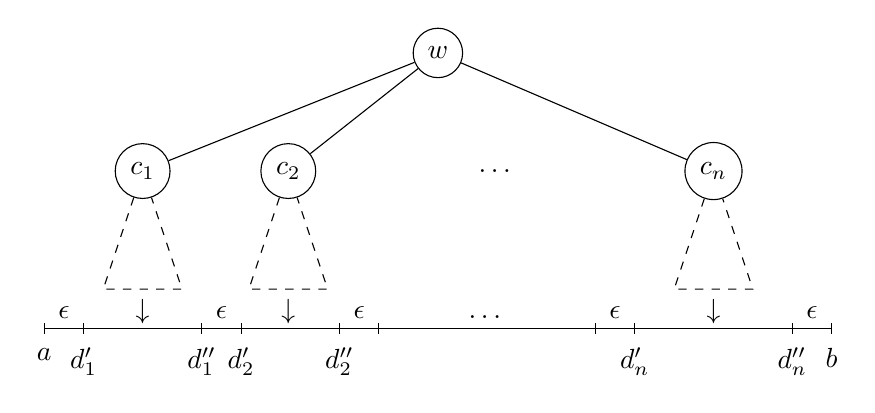
\begin{tikzpicture}[main/.style = {draw, circle}]
      \node [draw=none, label=below:$a$] (a) at (-5, -3.5) {};
      \node [draw=none, label=below:$b$] (b) at (5, -3.5) {};
      \draw (-5,-3.5) -- (5,-3.5);
      \node [draw=none, label=below:$d'_1$] (d1') at (-4.5, -3.5) {};
      \node [draw=none, label=below:$d''_1$] (d1'') at (-3, -3.5) {};
      \node [draw=none, label=below:$d'_2$] (d2') at (-2.5, -3.5) {};
      \node [draw=none, label=below:$d''_2$] (d2'') at (-1.25, -3.5) {};
      \node [draw=none] (d3') at (-.75, -3.5) {};
      \node [draw=none] (dn1'') at (2, -3.5) {};
      \node [draw=none, label=below:$d'_n$] (dn') at (2.5, -3.5) {};
      \node [draw=none, label=below:$d''_n$] (dn'') at (4.5, -3.5) {};
      \draw [draw=none] (a) -- node[midway, above] {$\epsilon$} (d1');
      \draw [draw=none] (d1'') -- node[midway, above] {$\epsilon$} (d2');
      \draw [draw=none] (d2'') -- node[midway, above] {$\epsilon$} (d3');
      \draw [draw=none] (dn1'') -- node[midway, above] {$\epsilon$} (dn');
      \draw [draw=none] (dn'') -- node[midway, above] {$\epsilon$} (b);
      \draw [draw=none] (d2'') -- node[midway, above] {$\dots$} (dn');

      \foreach \n in {a, b, d1', d1'', d2', d2'', d3', dn1'', dn', dn''}
               {
                 \draw ($ (\n) + (0, +2pt) $) -- ($ (\n) - (0, 2pt) $);
               }
      \node [main] (w) {$w$}
        child {node [main, xshift = -1.5cm] (c1) {$c_1$}}
        child {node [main, xshift = -1.15cm] (c2) {$c_2$}}
        child {node {$\dots$} edge from parent [draw=none]}
        child {node [main, xshift = 1.25cm] (cn) {$c_n$}};
        \foreach \n in {c1, c2, cn}
                 {
                   \draw [dashed] (\n) -- +(-.5,-1.5) -- node[midway, below] {$\downarrow$} +(.5,-1.5) -- (\n);
                 }
    \end{tikzpicture}
  \end{figure}

  Let $f_i$ be the preserving tree mapping from the induction hypothesis for $SubTree(T, c_i)$, $m \restriction V_{c_i}$ and $d'_{c_i}$ (the interval $[d'_{c_i}, d''_{c_i}]$). Now, we can define $f$:
  \begin{equation*}
    f \eqdef \langle w, p \rangle \cup \bigcup_{\mathclap{1 \leq i \leq n}}f_i
  \end{equation*}

  The domains of these functions are disjoint, so $f$ is a function from $V_w$ to $\Pol(\R)$. Clearly $a < d'_i < d''_i < d'_j < d''_j < b$ for $1 \leq i < j \leq n$, so
  \begin{equation*}
    (\forall u \in V_w)(f(u) \subseteq [a, b]).
  \end{equation*}
  Further,
  \begin{equation*}
    \bigcup_{\mathclap{u \in V_w}}f(u) = p \cup \bigcup_{\mathclap{1 \leq i \leq n}} [d'_i, d''_{i}] = [a, b]
  \end{equation*}
  and $a \in p = f(w)$, $b \in p = f(w)$.

  Now it remains to prove that $f$ is a preserving tree mapping.
  \begin{itemize}
  \item To show the parthood property, suppose $u_1 \in V_w$, $u_2 \in V_w$ and $u_1 \neq u_2$.
    \begin{itemize}
    \item If $u_1$ and $u_2$ are both in $V_{c_i}$ for some $i \in \{1, \dots n\}$, given that $f_i$ is a preserving tree mapping, $f(u_1) \bcap f(u_2) = f_i(u_1) \bcap f_i(u_2) = \emptyset$.
    \item If $u_1 \in V_{c_i}$ and $u_2 \in V_{c_j}$, for some $i, j \in \{1, \dots, n\}$ and $i \neq j$, then $f(u_1) = f_i(u_1) \subseteq [d'_i, d''_i]$ and $f(u_2) = f_j(u_2) \subseteq [d'_j, d''_j]$. $[d'_i, d''_i] \cap [d'_j, d''_j] = \emptyset$, so $f(u_1) \bcap f(u_2) \subseteq f(u_1) \cap f(u_2) = \emptyset$.
    \item If $u_1 = w$ or $u_2 = w$, without loss of generality, assume $u_1 = w$. Then $u_2 \in V_i$ for some $i \in \{1, \dots n\}$. Thus, $f(u_1) = p$ and $f(u_2) \subseteq [d'_i, d''_i]$.
      \begin{equation*}
        f(u_1) \bcap f(u_2) \subseteq f(u_1) \cap f(u_2) \subseteq p \cap [d'_i, d''_i] \subseteq \{d'_i, d''_i\}
      \end{equation*}
and so $f(u_1) \bcap f(u_2) = \emptyset$.
    \end{itemize}
  \item To show the contact property, suppose $u_1 \in V_w$, $u_2 \in V_w$ and $u_1 \neq u_2$.
    \begin{itemize}
    \item If $u_1$ and $u_2$ are both in $V_{c_i}$ for some $i \in \{1, \dots n\}$, $f(u_1) = f_i(u_1)$, $f(u_2) = f_i(u_2)$
      \begin{align*}
        \bcont(f(u_1), f(u_1)) &\leftrightarrow \bcont(f_i(u_1), f_i(u_1)) \equivih \\
        \{u_1, u_2\} \in E_{c_i} &\leftrightarrow \{u_1, u_2\} \in E_w.
      \end{align*}
    \item If $u_1 \in V_{c_i}$ and $u_2 \in V_{c_j}$, for some $i, j \in \{1, \dots, n\}$ and $i \neq j$, then $\{u_1, u_1\} \not \in E_w$. $f(u_1) = f_i(u_1) \subseteq [d'_i, d''_i]$, $f(u_2) = f_j(u_2) \subseteq [d'_j, d''_j]$. $[d'_i, d''_i] \cap [d'_j, d''_j] = \emptyset$, so $f(u_1) \cap f(u_2) = \emptyset$ and $\bcont(f(u_1), f(u_2))$ does not hold.
    \item If $u_1 = w$ or $u_2 = w$, without loss of generality, assume $u_1 = w$. Then $u_2 \in V_i$ for some $i \in \{1, \dots n\}$.
      \begin{align*}
        \{u_1, u_2\} \in E_W &\leftrightarrow \\
        u_2 = c_i &\equivih & (\text{looking at the Boolean} \\
        &&\text{disjoint polytopes in } [d'_i, d''_i]) \\
        d'_i \in f_i(c_i) &\leftrightarrow &(\text{considering the definition of p}) \\
        p \cap f_i(c_i) \neq \emptyset &\leftrightarrow \\
        f(u_1) \cap f(u_2) \neq \emptyset &\leftrightarrow \\
        \bcont(f(u_1), f(u_2)
      \end{align*}
    \end{itemize}
  \item For the measure property, simply note that it holds for $f_i$ and $u \in V_{c_i}$, where $i = 1, \dots, n$, by induction hypothesis and that
    \begin{equation*}
      \mu^\R(f(w)) = \mu^\R(p) \eqdef \epsilon + \epsilon + (n - 1)\epsilon = (n+1) \frac{m(w)}{n + 1} = m(w).
    \end{equation*}
  \end{itemize}
Finally, note that the given definition of $f$ is easily implemented in a procedure, $f$ is effectively constructable from $f_1, f_2, \dots, f_n$.
\end{proof}

Remark that $a \in f(r)$ in the lemma above means also that for all $u \in V \setminus \{r\}$, $a \not \in f(u)$. This is because if $a \in f(u)$, for some $u$, then an interval in the standard representation of $f(r)$ and an interval in the standard representation of $f(u)$ would both contain $a$. Since both intervals are of non-zero length, they would have a regular, closed intersection and therefore $f(r) \bcap f(u) \neq \emptyset$, which is not allowed by the definition of preserving tree mapping. This reasoning will also be implicitly used on other occasions in the rest of the text.

The result of the lemma is slightly generalized below to allow a different vertex in the tree to touch the right end of the interval.
\begin{lemma}[Tree Mapping to Interval, Arbitrary Right End]
    Let $T = \langle V, E \rangle$ be a rooted tree with root $r$. For any $m : V \rightarrow \R^+$, $s \in V$, $a \in \R$ and $b = a + \sum_{u \in V}m(u)$ there is an effective procedure to construct a preserving tree mapping $f$ of $\langle T, m \rangle$ such that:
  \begin{itemize}
  \item $\bigcup_{u \in V}f(u) = [a, b]$,
  \item $a \in f(r)$ and $b \in f(s)$.
  \end{itemize}
\end{lemma}
\begin{proof}
  If $r = s$, the previous lemma is directly applied.

  Suppose $r \neq s$ and $v_1, v_2, \dots, v_n = s$ are the vertices along the path from $r$ to $s$. Let
  \begin{equation*}
    \epsilon \eqdef \frac{\min\{v_1, v_2, \dots, v_n\}}{2}.
  \end{equation*}
  Consider the modification to $m$:
  \begin{equation*}
    m'(u) \eqdef
    \begin{cases}
      m(u) - \epsilon & \text{if } u \in \{v_1, v_2, \dots, v_n\} \\
      m(u) & \text{otherwise.}
    \end{cases}
  \end{equation*}
  Let $f'$ be the result of the application of the previous lemma to the same tree, but with the function $m'$ and for the interval $[a, a + m'(V)] = [a, b - n\epsilon]$.
  \begin{equation*}
    f(u) \eqdef
    \begin{cases}
      f'(u) \cup [b - (n - i + 1)\epsilon, b - (n - i)\epsilon] & \text{if } u = v_i, \text{ for } i \in \{1, 2, \dots, n\} \\
      f'(u) & \text{otherwise}
    \end{cases}
  \end{equation*}
  \begin{figure}[ht]
    \centering
    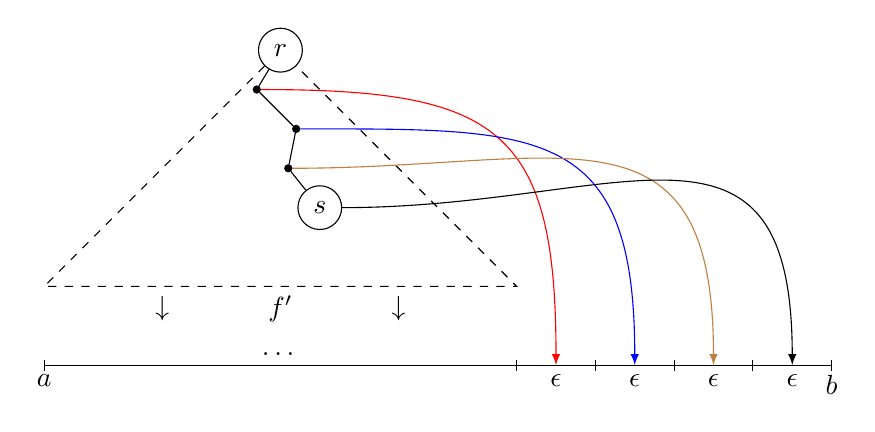
\begin{tikzpicture}[main/.style = {draw, circle}, v/.style = {circle, inner sep = 0pt, outer sep = 0pt, minimum size = 3pt, fill = black}, a/.style = {-latex}]
      \node [main] (r) at (-2, 0) {$r$};
      \node [v] (v1) at (-2.3, -.5) {};
      \node [v] (v2) at (-1.8, -1) {};
      \node [v] (v3) at (-1.9, -1.5) {};
      \node [main] (s) at (-1.5, -2) {$s$};
      \draw [] (r) -- (v1) -- (v2) -- (v3) -- (s);
      \draw [dashed] (r) -- +(-3,-3) -- node[pos=.25, below] {$\downarrow$} node[pos=.5, below] {$f'$} node[pos=.75, below] {$\downarrow$} +(3,-3) -- (r);

      \node [coordinate, label=below:$a$] (a) at (-5, -4) {};
      \node [coordinate, label=below:$b$] (b) at (5, -4) {};
      \draw (a) -- (b);
      \node [coordinate] (1) at (1, -4) {};
      \node [coordinate] (2) at (2, -4) {};
      \node [coordinate] (3) at (3, -4) {};
      \node [coordinate] (4) at (4, -4) {};

      \draw [draw=none] (1) -- node[coordinate, midway, label=below:$\epsilon$] (x1) {} (2);
      \draw [draw=none] (2) -- node[coordinate, midway, label=below:$\epsilon$] (x2) {} (3);
      \draw [draw=none] (3) -- node[coordinate, midway, label=below:$\epsilon$] (x3) {} (4);
      \draw [draw=none] (4) -- node[coordinate, midway, label=below:$\epsilon$] (xs) {} (b);

      \draw [a, red] (v1) to [out=0, in=90, looseness=1.5] (x1);
      \draw [a, blue] (v2) to [out=0, in=90, looseness=1.5] (x2);
      \draw [a, brown] (v3) to [out=0, in=90, looseness=1.5] (x3);
      \draw [a] (s) to [out=0, in=90, looseness=1.5] (xs);

      \draw [draw=none] (a) -- node[midway, above] {$\dots$} (1);

      \foreach \n in {a, b, 1, 2, 3, 4} {
        \draw ($ (\n) + (0, +2pt) $) -- ($ (\n) - (0, 2pt) $);
      }
    \end{tikzpicture}
  \end{figure}

  Clearly, for $1 \leq i < j \leq n$,
  \begin{align*}
    a &< b - n\epsilon \leq \\
    b - (n - i + 1)\epsilon &< b - (n - i)\epsilon \leq \\
    b - (n - j + 1)\epsilon &< b - (n - j)\epsilon \leq b.
  \end{align*}

  It can be seen by direct inspection that
  \begin{align*}
    &\bigcup_{u \in V}f(u) = [a, b], \\
    &a \in f(r) \text{ and } b \in f(s).
  \end{align*}

  \begin{itemize}
  \item To show the parthood and contact properties of $f$ simultaneously, consider $u_1, u_2 \in V$, $u_1 \neq u_2$.
    \begin{itemize}
    \item If both $u_1$ and $u_2$ are not in $\{r, v_1, \dots, v_n\}$, then $f(u_1) = f'(u_1)$ and $f(u_2) = f'(u_2)$ and the properties hold since $f'$ is a preserving tree mapping.
    \item If $u_1 \in \{r, v_1, \dots, v_n\}$, $u_2 \not\in \{r, v_1, \dots, v_n\}$ or vice-versa, then
      \begin{equation*}
        f(u_2) = f'(u_2) \subsetneq [a, b - n\epsilon] \text{, so } f(u_1) \cap f(u_2) \subseteq [a, b - n\epsilon].
      \end{equation*}
      Therefore,
      \begin{align*}
        f(u_1) \cap f(u_2) &= f'(u_1) \cap f'(u_2) \\
        f(u_1) \bcap f(u_2) &= f'(u_1) \bcap f'(u_2)
      \end{align*}
      and again the fact that $f'$ is a preserving tree mapping is used.
    \item If $u_1 = v_i$ and $u_2 = v_j$, without loss of generality, $i < j$.
      \begin{itemize}
      \item If $\{u_1, u_2\} \in E$, then $i + 1 = j$.
        \begin{align*}
          &f(u_1) \bcap f(u_2) \subseteq f(u_1) \cap f(u_2) = \\
          &(f'(u_1) \cap f'(u_2)) \cup \{b - (n - i)\epsilon\}.
        \end{align*}
        $f'(u_1) \cap f'(u_2)$ is finite, so $f(u_1) \bcap f(u_2) = \emptyset$. Also,
        \begin{equation*}
          b - (n - i)\epsilon \in f(u_1) \cap f(u_2) \text{, i.e. } \bcont(f(u_1), f(u_2)).
        \end{equation*}
      \item If $\{u_1, u_2\} \not\in E$, $f'(u_1) \cap f'(u_2) = \emptyset$, because $f'$ is a preserving tree mapping and
        \begin{equation*}
          (f(u_1) \cap f(u_2)) \cap [b - n\epsilon, b] = \emptyset,
        \end{equation*}
        so $f(u_1) \cap f(u_2) = \emptyset$ and of course $f(u_1) \bcap f(u_2) = \emptyset$.
      \end{itemize}
    \item To show the measure property for $u \in V$, consider two simple cases:
      \begin{itemize}
      \item if $u \in \{v_1, \dots, v_n\}$, then
        \begin{align*}
          \mu^\R(f(u)) &= \mu^\R(f'(u)) + \epsilon = \\
          m'(u) + \epsilon &= (m(u) - \epsilon) + \epsilon = \\
          &= m(u);
        \end{align*}
      \item otherwise, $\mu^\R(f(u)) = \mu^\R(f'(u)) = m'(u) = m(u)$.
      \end{itemize}
    \end{itemize}
  \end{itemize}
\end{proof}

The same idea is easily generalized to trees with an infinite root and half the real line.

\begin{lemma}[Tree Mapping to Half Line]
    Let $T = \langle V, E \rangle$ be a rooted tree with root $r$. For any $m : V \rightarrow \R^+ \cup \{\infty\}$ such that $(\forall v \in V)(m(v) = \infty \leftrightarrow v = r)$ and any $a \in \R$ there is an effective procedure to construct a preserving tree mapping $f$ of $\langle T, m \rangle$ such that:
  \begin{itemize}
  \item $\bigcup_{u \in V}f(u) = [a, \infty)$,
  \item $a \in f(r)$.
  \end{itemize}
\end{lemma}
\begin{proof}
  Let $c_1, c_2, \dots, c_n$ be the children of $r$. If $n = 0$, the entire mapping is $\{\langle r, [a, \infty) \rangle\}$. If not, let
  \begin{align*}
    a_i &\eqdef a + \sum_{j < i}\left(1 + m(SubTree(T, c_j))\right)\\
    b_i &\eqdef a_i + m(SubTree(T, c_i)),
  \end{align*} for $i \in \{1, \dots, n\}$. Let
  \begin{equation*}
    p \eqdef [a, a_1] \cup \bigcup_{\mathclap{1 \leq i \leq n}}[b_i, a_{i+1}]
  \end{equation*}

  \begin{figure}[ht]
    \centering
    \begin{tikzpicture}[main/.style = {draw, circle}]
      \node [draw=none, label=below:$a$] (a) at (-5, -3.5) {};
      \draw [-latex] (-5,-3.5) -- (6.5,-3.5);
      \node [draw=none, label=below:$a_1$] (d1') at (-4.5, -3.5) {};
      \node [draw=none, label=below:$b_1$] (d1'') at (-3, -3.5) {};
      \node [draw=none, label=below:$a_2$] (d2') at (-2.5, -3.5) {};
      \node [draw=none, label=below:$b_2$] (d2'') at (-1.25, -3.5) {};
      \node [draw=none] (d3') at (-.75, -3.5) {};
      \node [draw=none] (dn1'') at (2, -3.5) {};
      \node [draw=none, label=below:$a_n$] (dn') at (2.5, -3.5) {};
      \node [draw=none, label=below:$b_n$] (dn'') at (4.5, -3.5) {};
      \draw [draw=none] (a) -- node[midway, above] {$1$} (d1');
      \draw [draw=none] (d1'') -- node[midway, above] {$1$} (d2');
      \draw [draw=none] (d2'') -- node[midway, above] {$1$} (d3');
      \draw [draw=none] (dn1'') -- node[midway, above] {$1$} (dn');
      \draw [draw=none] (d3') -- node[midway, above] {$\dots$} (dn1'');

      \foreach \n in {a, d1', d1'', d2', d2'', d3', dn1'', dn', dn''}
               {
                 \draw ($ (\n) + (0, +2pt) $) -- ($ (\n) - (0, 2pt) $);
               }
      \node [main] (w) {$r$}
        child {node [main, xshift = -1.5cm] (c1) {$c_1$}}
        child {node [main, xshift = -1.15cm] (c2) {$c_2$}}
        child {node {$\dots$} edge from parent [draw=none]}
        child {node [main, xshift = 1.25cm] (cn) {$c_n$}};
        \foreach \n in {c1, c2, cn}
                 {
                   \draw [dashed] (\n) -- +(-.5,-1.5) -- node[midway, below] {$\downarrow$} +(.5,-1.5) -- (\n);
                 }
    \end{tikzpicture}
  \end{figure}

  We apply the (Tree Mapping to Interval, Root at Both Ends) lemma to each child $c_i$ ($i \in \{1, \dots, n\}$) and interval $[a_i, b_i]$ to get $f_1, f_2, \dots, f_n$ and define $f$:
  \begin{equation*}
    f(u) \eqdef
    \begin{cases}
      f_i(u) & \text{if } u \in SubTree(T, c_i), \text{ for some } i \in \{1, \dots, n\} \\
      p      & \text{if } u = r
    \end{cases}
  \end{equation*}

  The rest of the proof is analogous to the induction step of the proof of the (Tree Mapping to Interval, Root at Both Ends) lemma, except for the simplification of the measure of $f(r)$ being $\infty$.
\end{proof}
\begin{corollary}
The same can be done on the interval $(-\infty, a]$ by mirror symmetry.
\end{corollary}

\begin{lemma}[Relational Model Conversion]
  Let $S = \langle \B^W, \mathcal{C}^c, \leq_m \rangle$ be a convertible relational model and $v$ be a disjoint valuation. If $\phi$ is a formula from $\lang$ and $\langle S, v \rangle \models \phi$, then a valuation $v_\R: \Vars \rightarrow \Pol(\R)$ such that $\langle S^\R, v_\R \rangle \models \phi$ can be effectively constructed.
\end{lemma}
\begin{proof}
  $S$ is a convertible relational model, so by the corollary of the (Untying) lemma, let $S' = \langle \B^{W'}, \mathcal{C}^{c'}, \leq_{m'} \rangle$ and $v'$ be a convertible relational model and a valuation which model the same formulas and it holds that $Gr(S') = \langle V, E \rangle$ is a tree.

  Since $S'$ is convertible, there are exactly two vertices with infinite values for $m$.Let $i_1$ and $i_2$ be those vertices, $m(i_1) = m(i_2) = \infty$, and $i_1, w_1, w_2, \dots, w_n, i_2$ be the path from $i_1$ to $i_2$. The graph $\langle V, E \setminus \{\{i_1, w_1\}, \{w_n, i_2\}\} \rangle$ has three connected components: one containing $i_1$, one containing $w_1, \dots, w_n$ and one containing $i_2$. Let $\langle V_{i_1}, E_{i_1} \rangle$, $\langle V_w, E_v \rangle$ and $\langle V_{i_2}, E_{i_2} \rangle$ respectively be the trees induced by those components.

  Consider $\langle V_{i_1}, E_{i_1} \rangle$ and $\langle V_{i_2}, E_{i_2} \rangle$ as rooted trees with roots $i_1$ and $i_2$ respectively. They satisfy the conditions for the (Tree Mapping to Half Line) lemma and corollary (with $m \restriction V_{i_1}$ and $m \restriction V_{i_2}$). Thus, let $f_{i_1}$ be the mapping from the corollary for $\langle V_{i_1}, E_{i_1} \rangle$ and interval $(-\infty, 0]$ and $f_{i_2}$ be the mapping from the lemma for $\langle V_{i_1}, E_{i_1} \rangle$ and interval $[m(V_w), \infty)$.

    Now, consider $\langle V_w, E_v \rangle$ as a rooted tree with root $w_1$. The (Tree Mapping to Interval, Arbitrary Right End) lemma is applied to this rooted tree with $w_n$ in the role of the vertex $s$ (and $m \restriction V_w$), resulting in a preserving tree mapping $f_w$ onto the interval $[0, m(V_w)]$.

    \begin{figure}[ht]
      \centering
      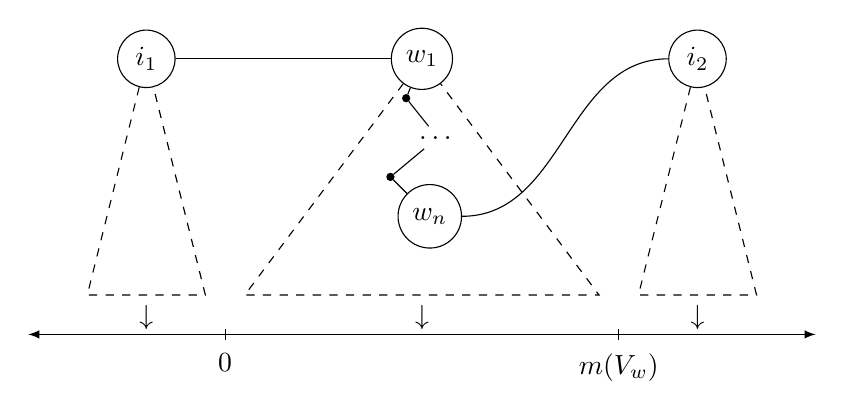
\begin{tikzpicture}[main/.style = {draw, circle}, v/.style = {circle, inner sep = 0pt, outer sep = 0pt, minimum size = 3pt, fill = black}]
        \draw [latex-latex] (-5,-3.5) -- (5,-3.5);

        \node [draw=none, label=below:$0$] (0) at (-2.5, -3.5) {};
        \node [draw=none, label=below:$m(V_w)$] (1) at (2.5, -3.5) {};

        \foreach \n in {0, 1}
                 {
                   \draw ($ (\n) + (0, +2pt) $) -- ($ (\n) - (0, 2pt) $);
                 }
                 \node [main] (i1) at (-3.5, 0) {$i_1$};
                 \node [main] (i2) at (3.5, 0) {$i_2$};

                 \node [main] (v1) at (0, 0) {$w_1$};
                 \node [v] (v2) at (-.2, -.5) {};
                 \node [] (v3) at (.2, -1) {$\dots$};
                 \node [v] (v4) at (-.4, -1.5) {};
                 \node [main] (vn) at (.1, -2) {$w_n$};
                 \draw [] (v1) -- (v2) -- (v3) -- (v4) -- (vn);
                 \draw [dashed] (v1) -- +(-2.25,-3) -- node[pos=.5, below] {$\downarrow$} +(2.25,-3) -- (v1);

                 \draw (i1) -- (v1);
                 \draw (vn) to [out=0, in=180, looseness = 1] (i2);
                 \foreach \n in {i1, i2}
                          {
                            \draw [dashed] (\n) -- +(-.75,-3) -- node[midway, below] {$\downarrow$} +(.75,-3) -- (\n);
                          }
      \end{tikzpicture}
    \end{figure}

    Of course, it should be noted that if $n = 0$, i.e. $i_1$ and $i_2$ are directly connected by an edge, then there would only be two connected components. In that case, $\langle V_w, E_v \rangle$ would be an empty graph. This poses no problem to the rest of the proof, as then $m(V_w) = 0$ and this empty graph would be mapped to a zero-length interval.

    Let $f = f_{i_1} \cup f_w \cup f_{i_2}$. First, it is useful to note that
    \begin{align*}
      & \bigcup_{i \in V}f(i) = \bigcup_{i \in V_{i_1}}f_{i_1}(i) \cup \bigcup_{i \in V_w}f_w(i) \cup \bigcup_{i \in V_{i_2}}f_{i_2}(i) = \\
      & (-\infty, 0] \cup [0, m(V_w)] \cup [m(V_w), \infty) = \R.
    \end{align*}
    Now follows a proof that $f$ is a preserving tree mapping of $\langle \langle V, E \rangle, m \rangle$.
    \begin{itemize}
    \item Let $u_1 \in V$ and $u_2 \in V$, $u_1 \neq u_2$.
      \begin{itemize}
      \item If $u_1$ and $u_2$ are in the same connected component of $\langle V, E \setminus \{\{i_1, w_1\}, \{w_n, i_2\}\} \rangle$, then the parthood and contact properties are satisfied for $f$ since $f_{i_1}$, $f_w$, and $f_{i_2}$ are preserving tree mappings.
      \item If $u_1$ is in one of $V_{i_1}$, $V_{i_2}$ and $u_2$ in the other, then $f(u_1) \subseteq (-\infty, 0]$ and $f(u_2) \subseteq [m(V_w), \infty)$ or vice-versa.
    Thus, $f(u_1) \cap f(u_2) = \emptyset$ is only possible if $V_w$ is empty ($n = 0$) and $\{u_1, u_2\} = \{i_1, i_2\}$, in which case $\{u_1, u_2\} \in E$. In any case, $f(u_1) \bcap f(u_2) = \emptyset$.
  \item Suppose $u_1$ is in $V_w$ and $u_2$ in $V_{i_1}$. Then $f(u_1) \subseteq (-\infty, 0]$ and $f(u_2) \subseteq [0, m(V_w)]$. Of course, $f(u_1) \bcap f(u_2) = \emptyset$. $f(u_1) \cap f(u_2)$ holds by construction of the lemma exactly if $u_1 = i_1$ and $u_2 = w_1$, in  which case $\{u_1, u_2\} \in E$.

    A similar argument is made if $u_1$ and $u_2$ switch places above or if $u_1$ is in $V_{i_2}$ and $u_2$ is in $V_w$ or the other way around.
      \end{itemize}
    \item For any $u \in V$, $u$ is in one of $V_{i_1}$, $V_w$ or $V_{i_1}$. In all three cases, $\mu^\R(f(u)) = m(u)$ since $f_{i_1}$, $f_w$ and $f_{i_2}$ are preserving tree mappings.
    \end{itemize}

    Let $v_\R(x) \eqdef \bigcup\{ f(i) \mid i \in v'(x) \}$. The proof that for any term $\tau$ of $\lang$, $v_\R^{S^\R}(\tau) = \bigcup\{ f(i) \mid i \in v'^{S'}(\tau)\}$ follows.

    For variables the statement is true by definition. For the constants:
    \begin{equation*}
      v_\R^{S^\R}(0) \eqdef \emptyset = \bigcup\{ f(i) \mid i \in \emptyset\} \eqdef \bigcup\{ f(i) \mid i \in v'^{S'}(0)\}
    \end{equation*}
    and
    \begin{align*}
      & v_\R^{S^\R}(1) \eqdef \R = (-\infty, 0] \cup [0, m(V_w)] \cup [m(V_w), \infty) = \\
    & \bigcup\{ f(i) \mid i \in V_{i_1}\} \cup \bigcup\{ f(i) \mid i \in V_w\} \cup \bigcup\{ f(i) \mid i \in V_{i_2}\} = \\
    & \bigcup\{ f(i) \mid i \in V\} \eqdef \bigcup\{ f(i) \mid i \in v'^{S'}(1)\}
    \end{align*}
Suppose that the statement is true for $\tau_1$ and $\tau_2$, terms of $\lang$. For the union operation:
    \begin{align*}
      & v_\R^{S^\R}(\tau_1 \lcup \tau_2) \eqdef v_\R^{S^\R}(\tau_1) \cup v_\R^{S^\R}(\tau_2) \eqih \\
      & \bigcup\{ f(i) \mid i \in v'^{S'}(\tau_1)\} \cup \bigcup\{ f(i) \mid i \in v'^{S'}(\tau_2)\} = \\
      & \bigcup\{ f(i) \mid i \in v'^{S'}(\tau_1 \lcup \tau_2)\}
    \end{align*}
    and for intersection:
    \begin{align*}
      & v_\R^{S^\R}(\tau_1 \lcap \tau_2) \eqdef v_\R^{S^\R}(\tau_1) \bcap v_\R^{S^\R}(\tau_2) \eqih \\
      & \bigcup\{ f(i) \mid i \in v'^{S'}(\tau_1)\} \bcap \bigcup\{ f(i) \mid i \in v'^{S'}(\tau_2)\} = & (\B^\R \text{is a Boolean algebra}) \\
      & \bigcup\{ f(i) \bcap \bigcup\{ f(j) \mid j \in v'^{S'}(\tau_2)\} \mid i \in v'^{S'}(\tau_1)\} = & (\B^\R \text{is a Boolean algebra}) \\
      & \bigcup\{ \bigcup\{ f(i) \bcap f(j) \mid j \in v'^{S'}(\tau_2)\} \mid i \in v'^{S'}(\tau_1)\} = & (\B^\R \text{is a Boolean algebra}) \\
      & \bigcup\{ f(i) \bcap f(j) \mid j \in v'^{S'}(\tau_2), i \in v'^{S'}(\tau_1)\} = & (f(i) \neq f(j) \rightarrow f(i) \bcap f(j) = \emptyset) \\
      & \bigcup\{ f(i) \mid i \in v'^{S'}(\tau_1) \cap v'^{S'}(\tau_2)\} \eqdef \\
      & \bigcup\{ f(i) \mid i \in v'^{S'}(\tau_1 \lcap \tau_2)\}
    \end{align*}
    For complement:
    \begin{align*}
      & v_\R^{S^\R}(\tau_1\lstar) \eqdef Cl(\R \setminus v_\R^{S^\R}(\tau_1)) \eqih Cl(\R \setminus \bigcup\{ f(i) \mid i \in v'^{S'}(\tau_1)\}) = \\
      & Cl\left(\left(\bigcup\{ f(i) \mid i \in v'^{S'}(\tau_1)\} \cup \bigcup\{ f(i) \mid i \in V \setminus v'^{S'}(\tau_1)\}\right) \setminus \bigcup\{ f(i) \mid i \in v'^{S'}(\tau_1)\}\right) = \\
      & Cl\left(\bigcup\{ f(i) \mid i \in V \setminus v'^{S'}(\tau_1)\} \setminus \bigcup\{ f(j) \mid j \in v'^{S'}(\tau_1)\}\right) = \\
      & Cl\left(\bigcup\left\{ f(i) \setminus \bigcup\{ f(j) \mid j \in v'^{S'}(\tau_1)\} \mid i \in V \setminus v'^{S'}(\tau_1)\right\}\right) = \\
      & Cl\left(\bigcup\left\{ \bigcap\{ f(i) \setminus f(j) \mid j \in v'^{S'}(\tau_1)\} \mid i \in V \setminus v'^{S'}(\tau_1)\right\}\right) = \\
      & \bigcup\left\{ Cl\left(\bigcap\{ f(i) \setminus f(j) \mid j \in v'^{S'}(\tau_1)\}\right) \mid i \in V \setminus v'^{S'}(\tau_1)\right\}
    \end{align*}
    Consider $f(i) \setminus f(j)$ in the above expression. $i \in V \setminus v'^{S'}(\tau_1)$ and $j \in v'^{S'}(\tau_1)$, so $i \neq j$. This means that $\emptyset = f(i) \bcap f(j) = Cl(Int(f(i) \cap f(j)))$, so \\
    $Int(f(i) \cap f(j)) = \emptyset$. Thus, $Int(f(i)) \subseteq f(i) \setminus f(j)$. From here, \\
    $Int(f(i)) \subseteq \bigcap\{ f(i) \setminus f(j) \mid j \in v'^{S'}(\tau_1)\}$ and applying $Cl$ to both sides, we get $Cl(Int(f(i))) \subseteq Cl\left(\bigcap\{ f(i) \setminus f(j) \mid j \in v'^{S'}(\tau_1)\}\right)$. Polytopes are regular closed sets, so $f(i) \subseteq Cl\left(\bigcap\{ f(i) \setminus f(j) \mid j \in v'^{S'}(\tau_1)\}\right)$. On the other hand, $Cl\left(\bigcap\{ f(i) \setminus f(j) \mid j \in v'^{S'}(\tau_1)\}\right) \subseteq Cl\left(\bigcap\{ f(i) \mid j \in v'^{S'}(\tau_1)\}\right) = Cl(f(i)) = f(i)$. Thus, $f(i) = Cl\left(\bigcap\{ f(i) \setminus f(j) \mid j \in v'^{S'}(\tau_1)\}\right)$ and by substituting in the last of the series of equations above, $v_\R^{S^\R}(\tau_1 \lcap \tau_2) = \bigcup\{ f(i) \mid i \in V \setminus v'^{S'}(\tau_1)\} \eqdef \bigcup\{ f(i) \mid i \in v'^{S'}(\tau_1\lstar)\}$.

    To finish the proof of the lemma, follows a proof by induction on the construction of $\phi$ that $\langle \B^\R, v_\R \rangle \models \phi \leftrightarrow \langle S', v' \rangle \models \phi$.
    \begin{itemize}
    \item For $\bot$ and $\top$, the statement is trivial.
    \item For $\tau_1 \lpart \tau_2$,
      \begin{align*}
        \langle \B^\R, v_\R \rangle \models \tau_1 \lpart \tau_2 &\leftrightarrow \\
        v_\R^{S^\R}(\tau_1) \subseteq v_\R^{S^\R}(\tau_2) &\leftrightarrow \\
        \bigcup\{f(i) \mid i \in v'^{S'}(\tau_1)\} \subseteq \bigcup\{f(i) \mid i \in v'^{S'}(\tau_2)\} &\leftrightarrow & (*) \\
        v'^{S'}(\tau_1) \subseteq v'^{S'}(\tau_2) &\leftrightarrow \\
        \langle S', v' \rangle \models \tau_1 \lpart \tau_2
      \end{align*}
      The equivalence at $(*)$ from right to left is direct.

      From left to right, first observe that for all $i, j \in V$, if $i \neq j$, then $Int(f(i)) \cap f(j) = \emptyset$. To show this, suppose the opposite: that $x \in Int(f(i)) \cap f(j)$. $x$ is an interior point for $f(i)$, so there must be a neighborhood $X$ of $x$, contained in $f(i)$. $x$ is in $f(j)$, a regular closed set, so $X$ contains an interior point $y$ of $f(j)$. Let $Y$ be a neighborhood of $y$, contained in $f(j)$. $y \in X \cap Y$, so $X \cap Y$ is a non-empty open set. $X \cap Y \subseteq f(i) \cap f(j)$, which is a contradiction with $Cl(Int(f(i) \cap f(j))) = \emptyset$.

      Bearing this in mind, let $i \in v'^{S'}(\tau_1)$. $Int(f(i)) \subseteq \bigcup\{f(i) \mid i \in v'^{S'}(\tau_1)\} \subseteq \bigcup\{f(i) \mid i \in v'^{S'}(\tau_2)\}$, so $i \in v'^{S'}(\tau_2)$ and $v'^{S'}(\tau_1) \subseteq v'^{S'}(\tau_2)$.
    \item For $\lcont(\tau_1, \tau_2)$,
      \begin{align*}
        \langle \B^\R, v_\R \rangle \models \lcont(\tau_1, \tau_2) &\leftrightarrow \\
        v_\R^{S^\R}(\tau_1) \cap v_\R^{S^\R}(\tau_2) \neq \emptyset &\leftrightarrow \\
        \bigcup\{f(i) \mid i \in v'^{S'}(\tau_1)\} \cap \bigcup\{f(i) \mid i \in v'^{S'}(\tau_2)\} \neq \emptyset &\leftrightarrow \\
        (\exists i \in v'^{S'}(\tau_1))(\exists j \in v'^{S'}(\tau_2))(f(i) \cap f(j) \neq \emptyset) &\leftrightarrow \\
        (\exists i \in v'^{S'}(\tau_1))(\exists j \in v'^{S'}(\tau_2))(\bcont(f(i), f(j))) &\leftrightarrow \\
        (\exists i \in v'^{S'}(\tau_1))(\exists j \in v'^{S'}(\tau_2))(\{i, j\} \in E) &\leftrightarrow \\
        v'^{S'}(\tau_1) \subseteq v'^{S'}(\tau_2) &\leftrightarrow \\
        \langle S', v' \rangle \models \lcont(\tau_1, \tau_2)
      \end{align*}
    \item For $\tau_1 \lmeasure \tau_2$,
      \begin{align*}
        \langle \B^\R, v_\R \rangle \models \tau_1 \lmeasure \tau_2 &\leftrightarrow \\
        \mu^\R(v_\R^{S^\R}(\tau_1)) \leq \mu^\R(v_\R^{S^\R}(\tau_2)) &\leftrightarrow \\
        \mu^\R\left(\bigcup\{f(i) \mid i \in v'^{S'}(\tau_1)\}\right) \leq \mu^\R\left(\bigcup\{f(i) \mid i \in v'^{S'}(\tau_2)\}\right) &\leftrightarrow TODO \\
        \sum_{\mathclap{i \in v'^{S'}(\tau_1)}}\mu^\R(f(i)) \leq \sum_{\mathclap{i \in v'^{S'}(\tau_2)}}\mu^\R(f(i)) &\leftrightarrow \\
        \sum_{\mathclap{i \in v'^{S'}(\tau_1)}}m(i) \leq \sum_{\mathclap{i \in v'^{S'}(\tau_2)}}m(i) &\leftrightarrow \\
        \langle S', v' \rangle \models \tau_1 \lmeasure \tau_2
      \end{align*}
    \end{itemize}
\end{proof}
\section{Axiomatization}
\subsection{Correctness}
\subsection{Completeness}
\end{document}
